\documentclass[final]{beamer}

% ====================
% Packages
% ====================

\usepackage[T1]{fontenc}
\usepackage{lmodern}
\usepackage[size=custom,width=120,height=72,scale=1.0]{beamerposter}
\usetheme{gemini}
\usecolortheme{cam}
\usepackage{graphicx}
\usepackage{booktabs}
\usepackage[numbers]{natbib}
\usepackage{tikz}
\usepackage{pgfplots}
\pgfplotsset{compat=1.14}
\usepackage{anyfontsize}

% ====================
% Lengths
% ====================

% If you have N columns, choose \sepwidth and \colwidth such that
% (N+1)*\sepwidth + N*\colwidth = \paperwidth
\newlength{\sepwidth}
\newlength{\colwidth}
\setlength{\sepwidth}{0.025\paperwidth}
\setlength{\colwidth}{0.3\paperwidth}

\newcommand{\separatorcolumn}{\begin{column}{\sepwidth}\end{column}}

% ====================
% Title
% ====================

\title{Rethinking Creditworthiness: Assessing Default Risk through Transaction Data}

\author{
    \makebox[0.2\textwidth]{Jevan Chahal} \hspace{0.5cm} 
    \makebox[0.2\textwidth]{Hillary Chang} \hspace{0.5cm} 
    \makebox[0.2\textwidth]{Kurumi Kaneko} \hspace{0.5cm}
    \makebox[0.2\textwidth]{Kevin Wong} \\[0.2cm]
    \makebox[0.2\textwidth]{\texttt{j2chahal@ucsd.edu}} \hspace{0.5cm} 
    \makebox[0.2\textwidth]{\texttt{hic001@ucsd.edu}} \hspace{0.5cm} 
    \makebox[0.2\textwidth]{\texttt{kskaneko@ucsd.edu}} \hspace{0.5cm} 
    \makebox[0.2\textwidth]{\texttt{kew024@ucsd.edu}} \\[0.3cm]
    {\small 
        \makebox[0.13\textwidth]{Mentor: Brian Duke} 
        \makebox[0.13\textwidth]{\texttt{brian.duke@prismdata.com}}
        \makebox[0.13\textwidth]{Kyle Nero}  
        \makebox[0.13\textwidth]{\texttt{kyle.nero@ucsd.edu}}
        \makebox[0.13\textwidth]{Berk Ustun}  
        \makebox[0.13\textwidth]{\texttt{berk@ucsd.edu}}
    }
}


% ====================
% Footer (optional)
% ====================

\footercontent{
  \href{https://github.com/hillarychang/dsc180b-capstone-q2}{https://github.com/hillarychang/dsc180b-capstone-q2} \hfill
  Link to Code and Website \hfill
  \href{https://hillarychang.github.io/dsc180b-capstone-q2/}{https://hillarychang.github.io/dsc180b-capstone-q2/}}

% ====================
% Logo (optional)
% ====================

% use this to include logos on the left and/or right side of the header:
\logoright{
\includegraphics[height=5cm]{logos/hdsi-white.png}}
%\logoleft{
\includegraphics[height=5cm]{logos/hdsi-blue-gold.png}}
% INCLUDE PRISM DATA LOGO

% ====================
% Body
% ====================

\begin{document}

\begin{frame}[t]
\begin{columns}[t]
\separatorcolumn

\begin{column}{\colwidth}

  \begin{block}{Background Information}

    Access to credit is crucial for financial stability, yet traditional credit scoring models often exclude individuals with limited credit history. The "Cash Score" project aims to address this issue by utilizing transaction data to evaluate financial behaviors rather than just historical credit data. Our goal is to provide a more equitable scoring system that benefits both consumers and financial institutions.

    We utilized multiple datasets that provide consumer transaction details, account balances, and delinquency indicators:
    \begin{itemize}
        \item \textbf{q2-ucsd-consDF.pqt}: Contains consumer attributes like \texttt{consumer\_id}, \texttt{credit\_score}, and \texttt{DQ\_target} (delinquency indicator).
        \item \textbf{q2-ucsd-acctDF.pqt}: Includes account-level data such as \texttt{consumer\_id}, \texttt{account\_id}, \texttt{balance\_date}, and \texttt{balance}.
        \item \textbf{q2-ucsd-trxnDF.pqt}: Captures transactional details including \texttt{category}, \texttt{amount}, \texttt{credit\_or\_debit}, and \texttt{posted\_date}.
        \item \textbf{categories.csv}: Maps transaction categories like Rent, Groceries, and Entertainment.
    \end{itemize}

  \end{block}

  \begin{block}{Research Question}

    How we can better measure a user’s credit worthiness such that we are more informed about their general decision-making and financial risk, with a consideration of risky behavior that has happened recently?

  \end{block}

  \begin{block}{Exploratory Data Analysis}

    \begin{itemize}
        \item Identified differences in transaction patterns between delinquent and non-delinquent consumers.
        \item Examined seasonal trends, payday effects, and spending fluctuations.
        \item Estimated income using recurring transactions.
        \item Analyzed the impact of account fees, buy-now-pay-later (BNPL) transactions, and overdrafts.
    \end{itemize}

    \textbf{Balance Trends for Delinquent Consumers}
    
    \begin{figure}[H]
        \centering
        \begin{minipage}{0.48\textwidth}
            \centering
            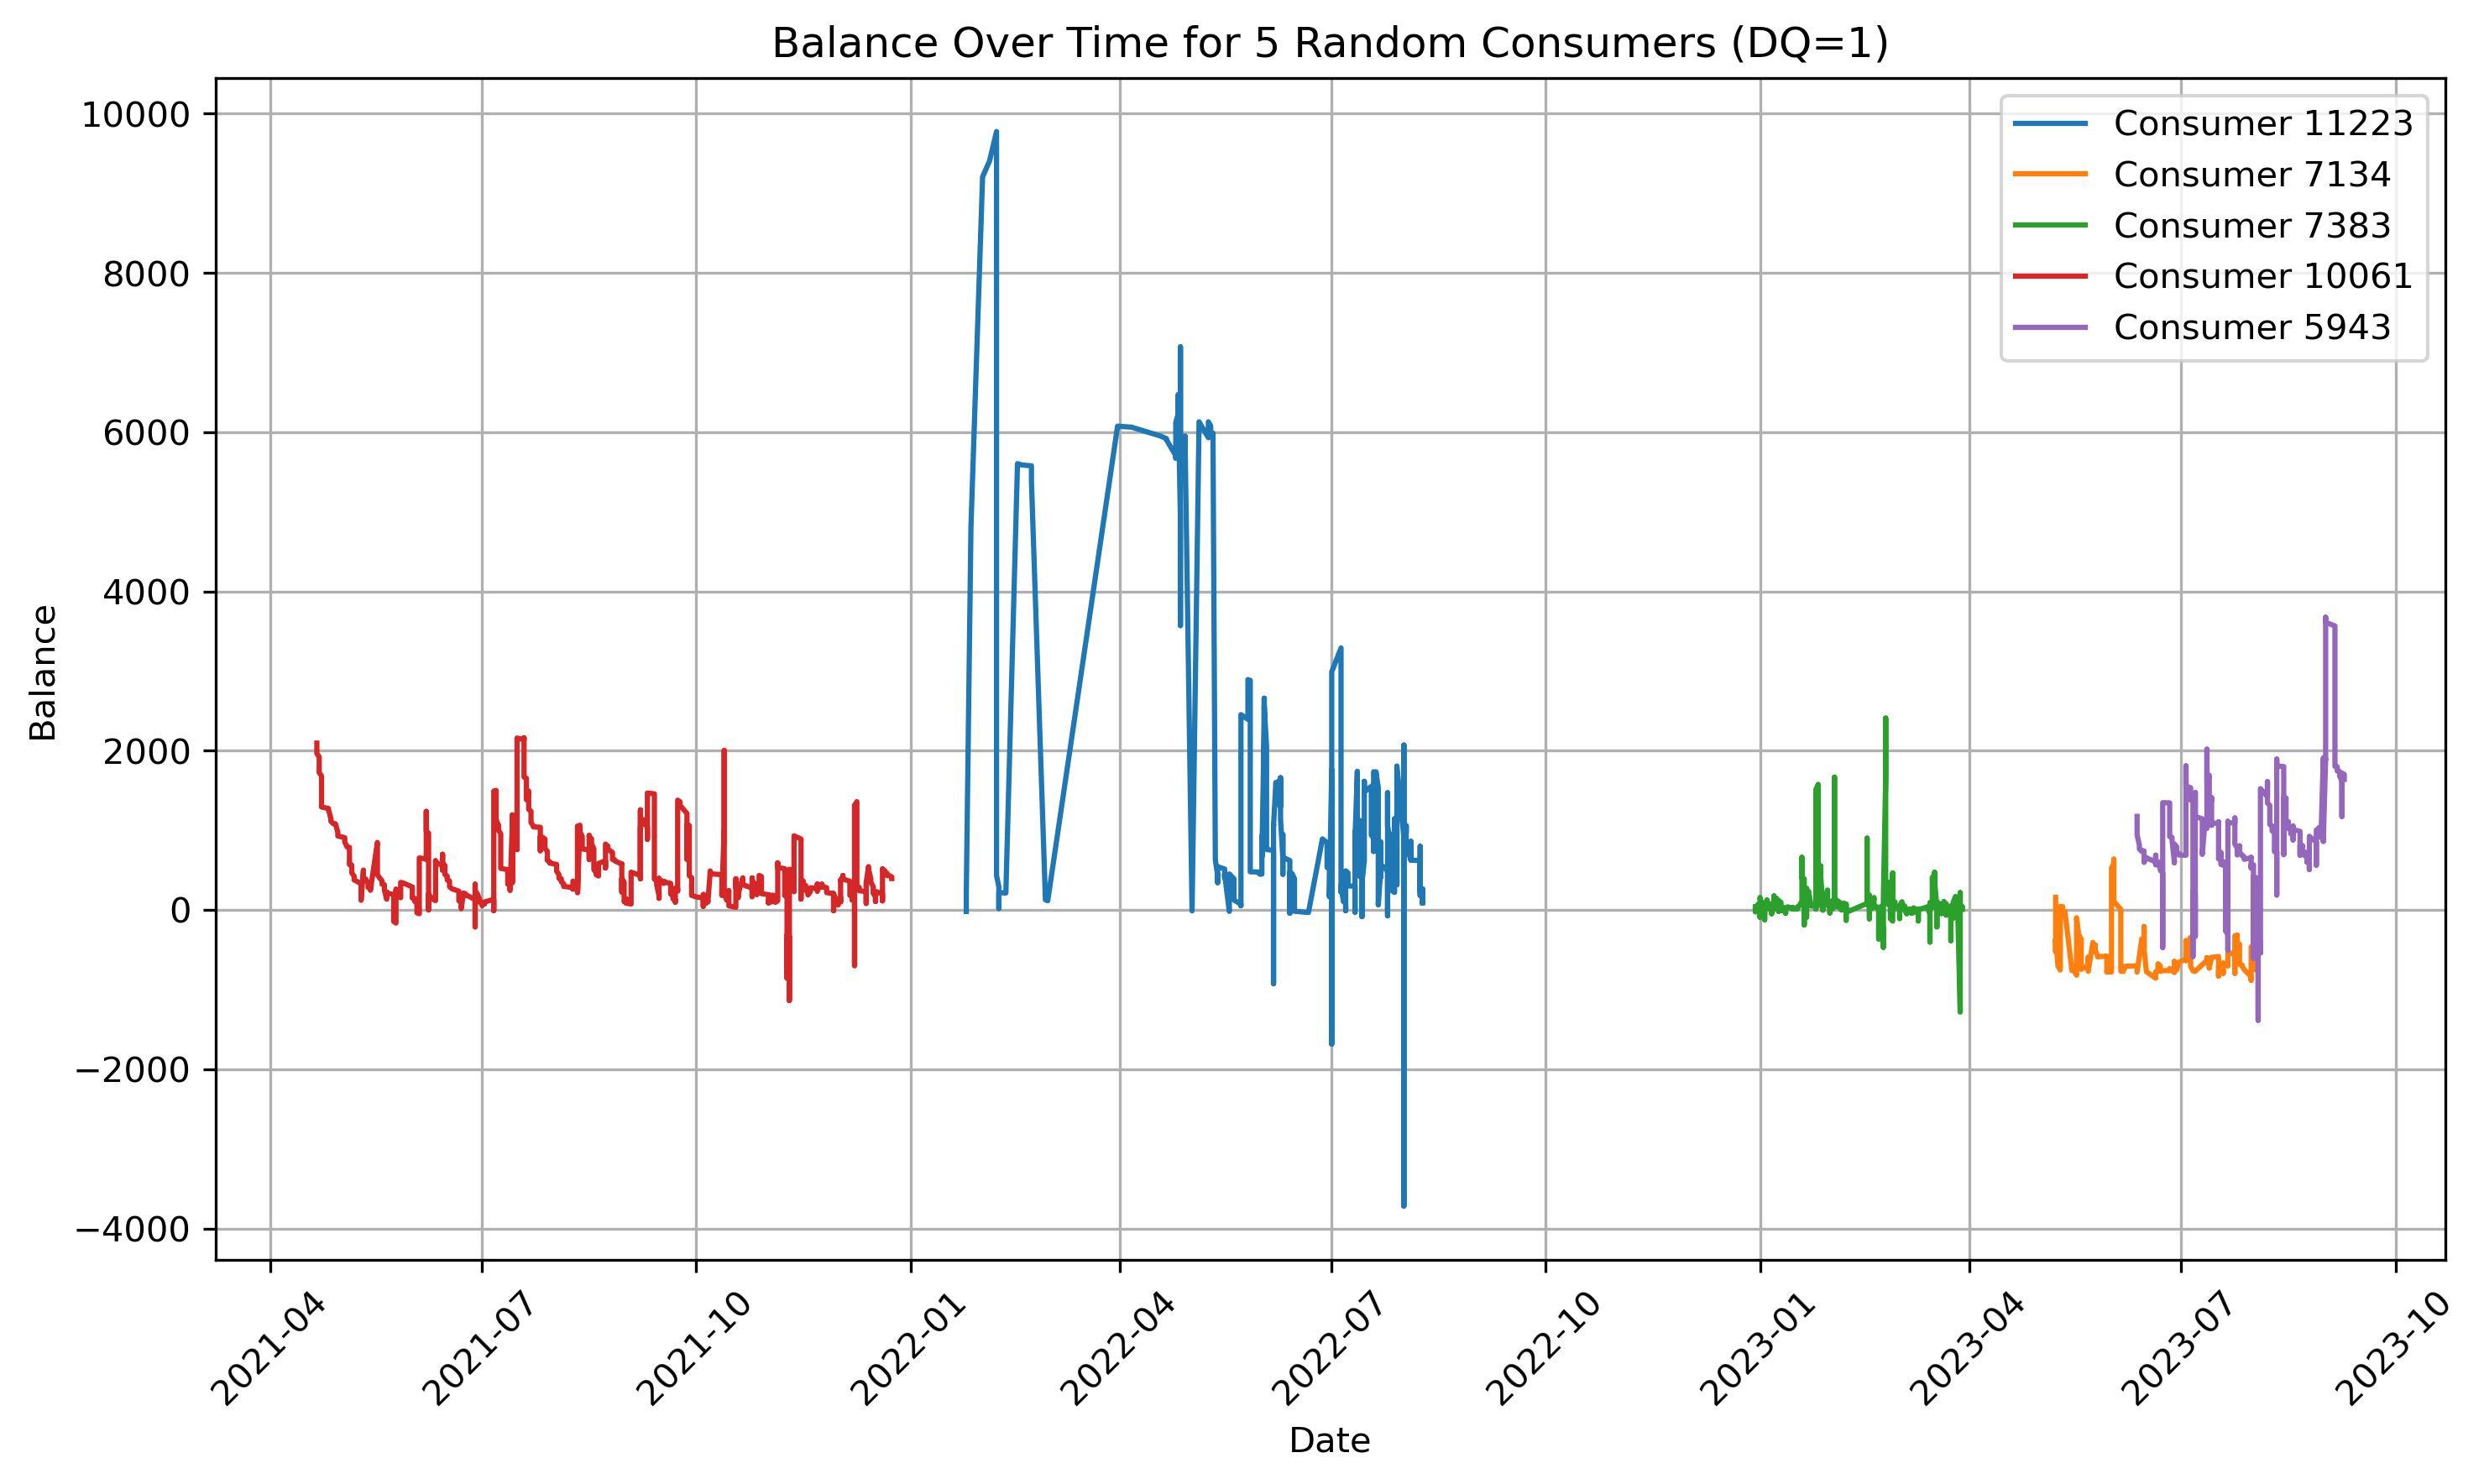
\includegraphics[width=\textwidth]{figure/balance_delinquent.png}
            \caption{Balance trends over time for five randomly selected delinquent consumers. The plot illustrates fluctuations and frequent occurrences of negative balances, highlighting financial instability.}
            \label{fig:balance_delinquent}
        \end{minipage}
        \hfill
        \begin{minipage}{0.48\textwidth}
            \centering
            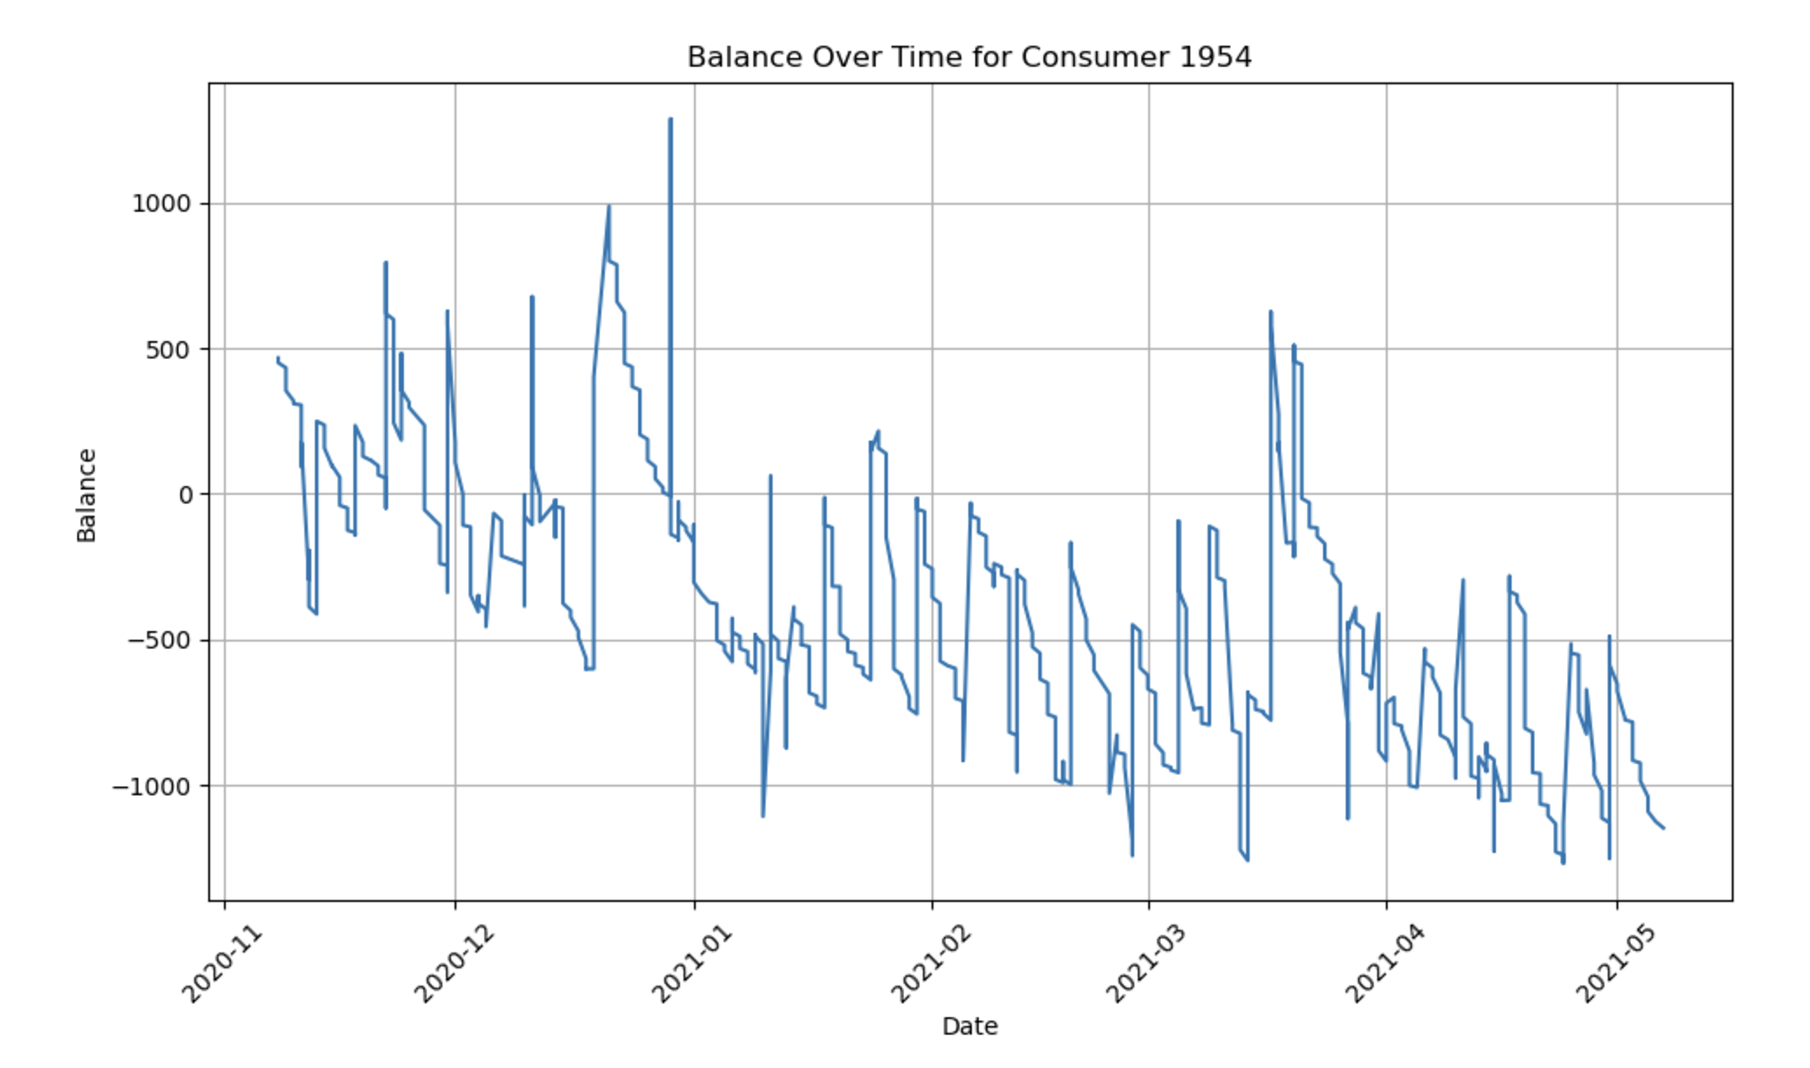
\includegraphics[width=\textwidth]{figure/balance_single_delinquent.png}
            \caption{Balance over time for a single delinquent consumer. This consumer frequently experiences negative balances, indicating financial distress and an increased risk of missing payments.}
            \label{fig:balance_single_delinquent}
        \end{minipage}
    \end{figure}

  \end{block}

  % \begin{alertblock}{A highlighted block}

  %   This block catches your eye, so \textbf{important stuff} should probably go

  % \end{alertblock}

\end{column}

\separatorcolumn

\begin{column}{\colwidth}

  \begin{block}{Feature Engineering}

    We engineered multiple features relevant to the prediction of delinquency:
    \begin{itemize}
        \item \textbf{Balance Features}: Negative balance ratio, balance trends, payday effects.
        \item \textbf{Transaction-Based Features}: Credit vs. debit transaction volume, category-based spending breakdown.
        \item \textbf{Temporal Features}: Spending frequency over time, account for longevity effects.
        \item \textbf{Account Types}: Features based on the types of accounts a consumer has
    \end{itemize}

    \begin{table}[H]
        \centering
        \begin{tabular}{|l|c|c|}
            \hline
            Feature & Importance & Correlation \\
            \hline
            account\_types\_savings & 0.044091 & -0.099071 \\
            account\_fees\_count & 0.037083 & 0.020680 \\
            credit\_score & 0.030284 & -0.249976 \\
            overdraft\_median & 0.026024 & 0.000407 \\
            account\_fees\_median & 0.021387 & 0.001497 \\
            BNPL\_std & 0.021323 & 0.034083 \\
            \hline
        \end{tabular}
        \caption{Top Features of XGBClassifier}
        \label{tab:top_features_xgb}
    \end{table}

  \end{block}

  \begin{block}{Model Evaluation}

    Key metrics for model evaluation include:
    \begin{itemize}
        \item \textbf{Accuracy and F1-Score}: Measures classification performance.
        \item \textbf{ROC-AUC}: Evaluates the model's ability to differentiate delinquent users.
        \item \textbf{Precision and Recall}: Precision measures correct positives; recall measures detected positives.
        \item \textbf{Training Time}: Time required to train the model.
        \item \textbf{Prediction Time}: Time taken to make predictions.
        \item \textbf{Feature Importance}: Highlights predictive variables.
    \end{itemize}
    To mitigate the class imbalance (delinquents only ~8.4\% of dataset), we used:
    \begin{itemize}
        \item \textbf{SMOTE \& SMOTEENN}: Oversampling techniques.
        \item \textbf{Feature Normalization}: Standardization of key variables.
    \end{itemize}

\vspace{1em}

\begin{columns}
\begin{column}{0.5\textwidth}  %%<--- here
\justify
WRITE DESCRIPTION HERE

\end{column}
\begin{column}{0.5\textwidth}
\begin{center}
      \begin{figure}[H]
        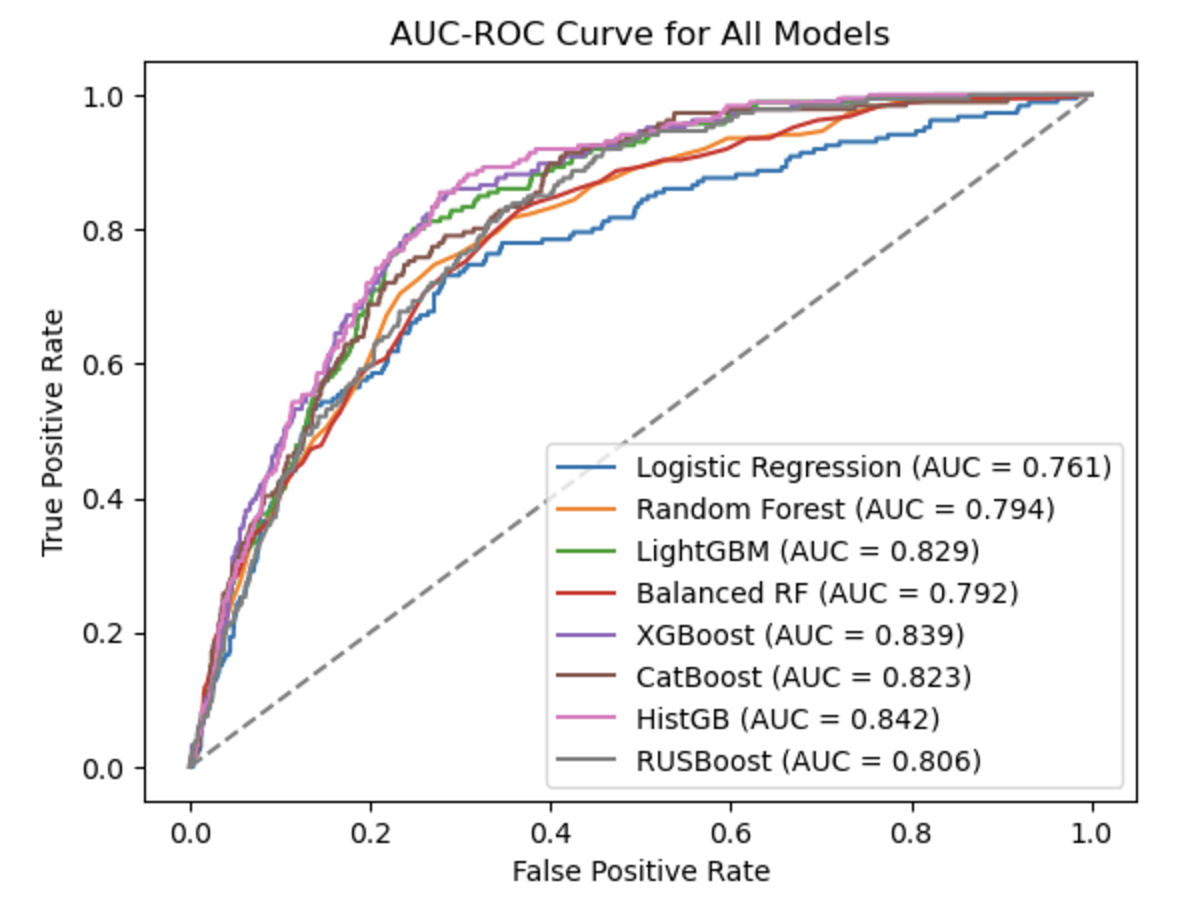
\includegraphics[width=\textwidth]{figure/auc_roc_all_models.png}
        \caption{All AUC-ROC scores for models we tested}
        \label{fig:accounts_df}
    \end{figure}
\end{center}
\end{column}
\end{columns}
  \end{block}
\end{column}

\separatorcolumn

\begin{column}{\colwidth}

  \begin{exampleblock}{Results}
\\
    \begin{center}
      \begin{figure}[H]
        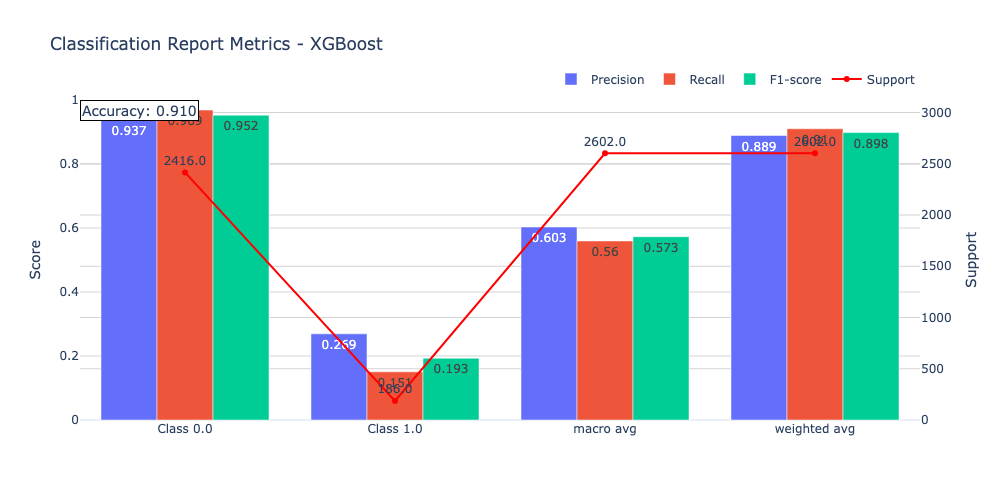
\includegraphics[width=0.4\textwidth]{figure/classification_report_xgboost.png}
        \caption{All AUC-ROC scores for models we tested}
        \label{fig:accounts_df}
      \end{figure}
    \end{center}
    
    \begin{table}[H]
    \centering
    \begin{tabular}{|l|c|c|c|c|c|c|c|}
        \hline
        Model & ROC-AUC & Accuracy & Precision & Recall & F1-Score \\
        \hline

        HistGB & \textbf{0.842428} & 0.913528 & 0.889776 & 0.913528 & 0.899533 \\
        XGBoost & 0.839279 & 0.910069 & 0.889033 & 0.910069 & 0.898105 \\
        LightGBM & 0.828857 & 0.913912 & 0.889361 & 0.913912 & 0.899373 \\
        CatBoost & 0.823153 & 0.915834 & 0.887905 & 0.915834 & 0.898882 \\
        RUSBoost & 0.805893 & 0.826287 & 0.905010 & 0.826287 & 0.857906 \\
        Random Forest & 0.794283 & 0.915450 & 0.885290 & 0.915450 & 0.897285 \\
        Balanced RF & 0.791598 & \textbf{0.919677} & 0.892594 & \textbf{0.919677} & \textbf{0.902200} \\
        Logistic Regression & 0.761125 & 0.759416 & \textbf{0.906664} & 0.759416 & 0.814041 \\
        \hline
    \end{tabular}
    \caption{Comparison of model performance}
    \end{table}

    STILL IN PROGRESS

  \end{exampleblock}

  \begin{block}{Conclusion}

    STILL IN PROGRESS

  \end{block}

  \begin{block}{References}

    \nocite{*}
    %\footnotesize{\bibliographystyle{plainnat}\bibliography{poster}}
    % ADD QR CODE AND OTHER LINKS

  \end{block}

\end{column}

\separatorcolumn
\end{columns}
\end{frame}

\end{document}
